\documentclass[dvisvgm,tikz,margin=2pt]{standalone}
\usepackage{amsmath,amssymb,amsthm,mathtools}
\usepackage{tikz}
\usetikzlibrary{positioning,calc}
\usepackage{xcolor}
\newcommand{\R}{\mathbb{R}}
\newcommand{\Q}{\mathbb{Q}}
\newcommand{\abs}[1]{\lvert #1\rvert}
\newcommand{\norm}[1]{\lVert #1\rVert}
\newcommand{\RSSP}{\textsc{Riesz-Subset}}
\newcommand{\MIS}{\textsc{Independent-Set}}
\newcommand{\sgnspin}{\{-1,+1\}}
\begin{document}
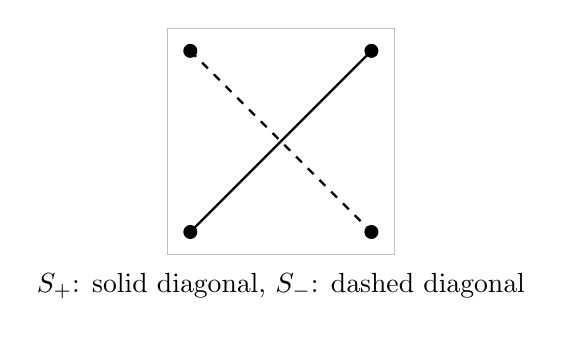
\begin{tikzpicture}[scale=1.15]
  \draw[gray!50] (-1.25,-1.25) rectangle (1.25,1.25);
  \fill (-1,-1) circle (2.2pt); \fill (1,1) circle (2.2pt);
  \fill (-1,1) circle (2.2pt); \fill (1,-1) circle (2.2pt);
  \draw[thick] (-1,-1)--(1,1);
  \draw[thick,dashed] (-1,1)--(1,-1);
  \node at (0,-1.6) {$S_+$: solid diagonal, $S_-$: dashed diagonal};
\end{tikzpicture}
\end{document}
